\باب{فوریئر تجزیہ}
\اصطلاح{دوری تفاعل}\فرہنگ{دوری!تفاعل}\فرہنگ{تفاعل!دوری}\حاشیہب{periodic function}\فرہنگ{periodic!function} سے مراد وہ تفاعل ہے جو درج ذیل مساوات پر پورا اترتا ہے جہاں \عددی{T_0}  \اصطلاح{دوری عرصہ}\فرہنگ{دوری عرصہ}\حاشیہب{time period}\فرہنگ{time period} کہلاتی ہے۔
\begin{align}
f(t)=f(t+nT_0), \quad n=\mp 1, \mp 2, \mp3, \cdots
\end{align}
درج بالا مساوات کہتی ہے کہ  کسی بھی لمحہ \عددی{t} پر دوری تفاعل کی قیمت \عددی{f(t)} اور اس لمحے سے \عددی{T_0} وقت بعد تفاعل کی قیمت \عددی{f(t+T_0)} برابر ہیں۔شکل \حوالہ{شکل_فوریئر_دوری_عرصہ} میں اس کی وضاحت  کی گئی ہے۔
\begin{figure}
\centering
\begin{tikzpicture}
\begin{axis}[kStyleCircuitsA,xtick={115,475},xticklabels={$t$,$t+T_0$},ytick=\empty]
\pgfmathsetmacro{\kt}{115}
\pgfmathsetmacro{\ktt}{\kt+360}
\addplot[domain=0:720,samples=100]{sin(x)+1/3*sin(3*x)};
\addplot[] plot coordinates {(\kt,{sin(\kt)+1/3*sin(3*\kt)+0.1}) (\kt,{sin(\kt)+1/3*sin(3*\kt)+0.3})};
\addplot[] plot coordinates {(\ktt,{sin(\ktt)+1/3*sin(3*\ktt)+0.1}) (\ktt,{sin(\ktt)+1/3*sin(3*\ktt)+0.3})};
\addplot[stealth-stealth] plot coordinates {(\kt,{sin(\kt)+1/3*sin(3*\kt)+0.2}) (\ktt,{sin(\ktt)+1/3*sin(3*\ktt)+0.2})}node[pos=0.5,fill=white]{$T_0$};
\addplot[] plot coordinates {(\kt,{sin(\kt)+1/3*sin(3*\kt)})}node[circ]{};
\addplot[] plot coordinates {(\ktt,{sin(\ktt)+1/3*sin(3*\ktt)})}node[circ]{};
\end{axis}
\end{tikzpicture}
\caption{دوری عرصہ۔}
\label{شکل_فوریئر_دوری_عرصہ}
\end{figure}
دوری عرصے کو سیکنڈ \عددی{(\si{\second})} میں ناپا جاتا ہے۔دوری عرصہ \عددی{T_0} اور \اصطلاح{تعدد}\فرہنگ{تعدد} \عددی{f_0} کا تعلق درج ذیل ہے جہاں تعدد کو \اصطلاح{ہرٹز}\فرہنگ{ہرٹز}\حاشیہب{Hertz, \si{\hertz}}\فرہنگ{Hertz}\فرہنگ{\si{\hertz}} \عددی{(\si{\hertz})} میں ناپا جاتا ہے۔
\begin{align}
f_0=\frac{1}{T_0}
\end{align}
\اصطلاح{زاویائی تعدد}\فرہنگ{زاویائی تعدد}\فرہنگ{تعدد!زاویائی} \عددی{\omega_0} اور تعدد \عددی{f_0} کا تعلق درج ذیل ہے۔
\begin{align}
\omega_0=2\pi f_0
\end{align}
زاویائی تعدد کو ریڈیئن فی سیکنڈ \عددی{(\si{\radian \per\second})} میں ناپا جاتا ہے۔شکل \حوالہ{شکل_فوریئر_چند_دوری_امواج} میں چند \اصطلاح{دوری امواج}\فرہنگ{دوری!موج}\فرہنگ{موج!دوری}\حاشیہب{periodic wave}\فرہنگ{periodic!wave} دکھائے گئے ہیں۔
\begin{figure}
\centering
\begin{subfigure}{0.5\textwidth}
\centering
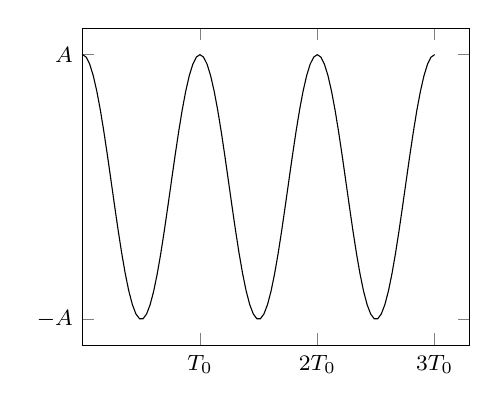
\begin{tikzpicture}
\begin{axis}[small,xmin=0,xtick={360,720,1080},xticklabels={$T_0$, $2T_0$,$3T_0$},ytick={-1,1},yticklabels={$-A$,$A$}]
\addplot[domain=0:1080,samples=100]{cos(x)};
\end{axis}
\end{tikzpicture}
\caption*{(الف) سائن نما موج۔}
\end{subfigure}%
\begin{subfigure}{0.5\textwidth}
\centering
\begin{tikzpicture}
\begin{axis}[small,xmin=0,xtick={1,3,6},xticklabels={$T_a$, $T_0$,$2T_0$},ytick={1},yticklabels={$A$}]
\addplot[] plot coordinates {(0,0) (0,1) (1,1) (1,0) (3,0) (3,1) (4,1) (4,0)(6,0) (6,1) (7,1) (7,0)};
\end{axis}%
\end{tikzpicture}
\caption*{(ب) مستطیل موج۔}
\end{subfigure}
\begin{subfigure}{0.5\textwidth}
\centering
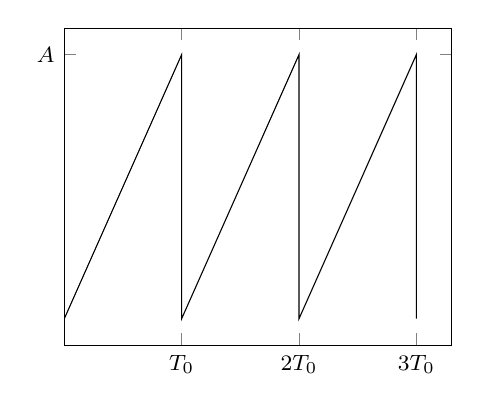
\begin{tikzpicture}
\begin{axis}[small,xmin=0,xtick={3,6,9},xticklabels={$T_0$, $2T_0$,$3T_0$},ytick={1},yticklabels={$A$}]
\addplot[] plot coordinates {(0,0) (3,1) (3,0) (6,1) (6,0) (9,1) (9,0)};
\end{axis}%
\end{tikzpicture}
\caption*{(پ) دندان موج۔}
\end{subfigure}%
\begin{subfigure}{0.5\textwidth}
\centering
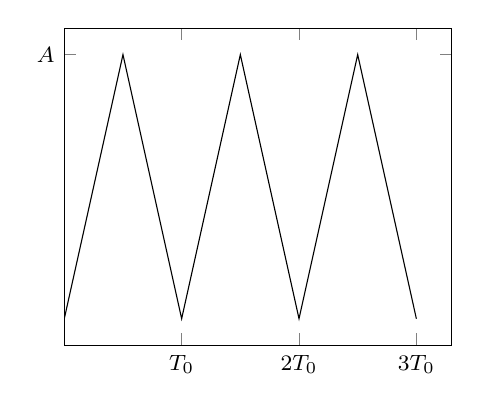
\begin{tikzpicture}
\begin{axis}[small,xmin=0,xtick={2,4,6},xticklabels={$T_0$, $2T_0$,$3T_0$},ytick={1},yticklabels={$A$}]
\addplot[] plot coordinates {(0,0) (1,1) (2,0) (3,1) (4,0) (5,1) (6,0)};
\end{axis}%
\end{tikzpicture}
\caption*{(ت) تکونی موج۔}
\end{subfigure}%
\caption{چند دوری امواج۔}
\label{شکل_فوریئر_چند_دوری_امواج}
\end{figure}

کسی بھی دوری تفاعل کو بطور درج ذیل (تکونیاتی) \اصطلاح{فوریئر تسلسل}\فرہنگ{فوریئر تسلسل!تکونیاتی}\فرہنگ{تسلسل!فوریئر}\حاشیہب{trignometric Fourier series}\فرہنگ{Fourier series!trignometric} لکھا\حاشیہد{جین بپٹسٹ یوسف فوریئر نے حرارتی توانائی کے بہاو پر غور کے دوران اس تسلسل کو دریافت کیا۔} جا سکتا ہے
\begin{gather}
\begin{aligned}\label{مساوات_فوریئر_تسلسل_سائن_نما_الف}
f(t)&=a_0+\sum_{n=1}^{\infty} [a_n \cos (n \omega_0 t) +b_n \sin (n \omega_0 t)]\\
&=a_0+a_1\cos \omega_0 t+a_2 \cos (2\omega_0 t)+a_3\cos (3\omega_0 t)+\cdots\\
&\phantom{=a_0\,\,}+b_1\sin \omega_0t+b_2\sin (2\omega_0t)+b_3 \sin (3\omega_0t)+\cdots
\end{aligned}
\end{gather}
جہاں \عددی{a_0}، \عددی{a_1}،\عددی{a_2}، \عددی{b_1} وغیرہ تسلسل کے \اصطلاح{عددی سر}\فرہنگ{عددی سر}\حاشیہب{coefficients}\فرہنگ{coefficients} کہلاتے ہیں۔فوریئر تسلسل کی اوسط قیمت \عددی{a_0} کے برابر ہے۔ایک دوری عرصہ \عددی{T_0} میں \عددی{\cos \omega_0 t} یا \عددی{\sin \omega_0 t} کی ایک لہر، \عددی{\cos (2\omega_0 t)} یا \عددی{\sin (2\omega_0 t)} کی دو لہریں اور \عددی{\cos (m\omega_0 t)} یا \عددی{\sin (m\omega_0 t)} کی \عددی{m} لہریں پوری آتی ہیں۔اس حقیقت کو شکل \حوالہ{شکل_فوریئر_ارکان_تعداد_فی_دوری_عرصہ} میں دکھایا گیا ہے جہاں وضاحت کی خاطر امواج کے حیطے مختلف رکھے گئے ہیں۔فوریئر تسلسل میں \عددی{a_1\cos \omega_0 t +b_1\sin \omega_0 t} \اصطلاح{بنیادی رکن}\فرہنگ{بنیادی رکن}\فرہنگ{ہارمونی!بنیادی رکن}\حاشیہب{fundamental component}\فرہنگ{fundamental component} یا \اصطلاح{پہلا ہارمونی رکن} کہلاتا ہے،   \عددی{a_2\cos (2\omega_0 t) +b_2\sin (2\omega_0 t)} \اصطلاح{دوسرا ہارمونی رکن}\فرہنگ{دوسرا ہارمونی رکن}\فرہنگ{ہارمونی!دوسرا رکن}\حاشیہب{second harmonic}\فرہنگ{harmonic!second} کہلاتا ہے،  \عددی{a_3\cos (3\omega_0 t) +b_3\sin (3\omega_0 t)} تیسرا ہارمونی رکن اور اسی طرح \عددی{a_m\cos (m\omega_0 t) +b_m\sin (m\omega_0 t)} ایم ہارمونی رکن کہلاتا ہے۔
\begin{figure}
\centering
\begin{tikzpicture}
\begin{axis}[kStyleCircuitsA,xlabel={$t\,(\si{\second})$},xtick={90,180,270,360},xticklabels={$\frac{1}{4}T_0$,$\frac{1}{2}T_0$,$\frac{3}{2}T_0$,$T_0$},ytick={1,-1},yticklabels={$+A_0$,$-A_0$}]
\addplot[mark=none,color=black,domain=0:360,samples=100]{sin(x)}node[pos=0.4,pin=45:{$A_0\sin \omega_0 t$}]{};
\addplot[mark=none,color=black,domain=0:360,samples=100]{0.5*sin(2*x)}node[pos=0.7,pin=45:{$\frac{A_0}{2}\sin 2\omega_0 t$}]{};
\end{axis}
\end{tikzpicture}
\caption{ایک دوری عرصہ میں فوریئر تسلسل کے ارکان کی تعداد۔}
\label{شکل_فوریئر_ارکان_تعداد_فی_دوری_عرصہ}
\end{figure}
%======================
ہم یہاں اصل رک کر چند حقائق اور تکملات پر غور کرتے ہیں جو فوریئر تسلسل میں کلیدی کردار ادا کرتے ہیں۔

آپ دو سمتیوں کے \اصطلاح{نقطہ ضرب}\فرہنگ{نقطہ ضرب}\فرہنگ{ضرب!نقطہ}\حاشیہب{dot product}\فرہنگ{dot product} سے خوب واقف ہیں۔سمتیہ \سمتیہ{A} اور \سمتیہ{B} کا نقطہ ضرب یا \اصطلاح{غیر سمتی ضرب}\فرہنگ{غیر سمتی ضرب}\فرہنگ{ضرب!غیر سمتی}\حاشیہب{scalar product}\فرہنگ{scalar product} درج ذیل ہے جہاں دونوں سمتیوں کے مابین زاویہ \عددی{\theta} ہے۔
\begin{align}
\kvec{A} \cdot \kvec{B}=A B \cos \theta
\end{align} 
آپس میں \اصطلاح{عمودی}\فرہنگ{عمودی}\حاشیہب{orthogonal}\فرہنگ{orthogonal} سمتیوں کے مابین \عددی{\theta=90^{\circ}} ہونے کی بدولت \عددی{\kvec{A} \cdot \kvec{B}=0} ہوتا ہے جبکہ کسی بھی سمتیہ کے خود نقطہ ضرب کا جذر اس کے حیطے  کے برابر ہوتا ہے۔
\begin{gather}
\begin{aligned}
 \abs{\kvec{A}}=\sqrt{\kvec{A} \cdot \kvec{A}}
\end{aligned}
\end{gather}
اسی سوچ کے ساتھ تفاعل کا نقطہ ضرب بیان کیا جاتا ہے۔

اگر تفاعل \عددی{f(t) \ne 0} اور \عددی{g(t)\ne 0} کے حاصل ضرب کا تکمل \عددی{a \le t \le b} فاصلے پر صفر کے برابر ہو
\begin{align}
\int_a^b f(t)g(t) \dif t=0
\end{align}
تو \عددی{a\le t\le b} فاصلے پر ان تفاعل کو آپس میں \اصطلاح{عمودی} تصور کیا جاتا ہے۔یاد رہے کہ دونوں تفاعل از خود \اصطلاح{غیر سمتی}\فرہنگ{غیر سمتی}\حاشیہب{scalar}\فرہنگ{scalar} اور غیر صفر ہیں۔

کسی بھی مقدار کا مربع مثبت ہوتا ہے لہٰذا تفاعل کا مربع \عددی{f^2(t)} ہر نقطے پر مثبت ہو گا۔ فاصلہ \عددی{a \le t \le b}  پر تفاعل کے \اصطلاح{معیار}\فرہنگ{معیار}\حاشیہب{norm}\فرہنگ{norm} \عددی{\parallel f(t) \parallel} سے مراد 
\begin{align}
\parallel f(t) \parallel =\sqrt{\int_a^b f^2(t) \dif t}
\end{align}
ہے۔
%===================
\ابتدا{مثال}
ثابت کریں کہ \عددی{0 \le t \le T_0}  فاصلے پر \عددی{\cos (m\omega_0 t)} اور \عددی{\cos (n\omega_0 t)} آپس میں عمودی ہیں جہاں \عددی{m=1,2,3,\cdots} اور \عددی{n=1,2,3,\cdots} ممکن ہیں لیکن \عددی{m\ne n} ہے۔

حل:دیے گئے فاصلے پر دونوں تفاعل کے حاصل ضرب کا تکمل لیتے ہیں۔
\begin{align*}
\int_0^{T_0} \cos (m\omega_0 t) \cos (n\omega_0 t) \dif t&=\int_0^{T_0} \frac{\cos\left[(m+n)\frac{2\pi}{T_0} t\right]+\cos\left[(m-n)\frac{2\pi}{T_0} t\right]}{2}\dif t\\
&=\left.\frac{\sin\left[(m+n)\frac{2\pi}{T_0} t\right]}{2(m+n)\frac{2\pi}{T_0} }+\frac{\sin\left[(m-n)\frac{2\pi}{T_0} t\right]}{2(m-n)\frac{2\pi}{T_0} }\right|_0^{T_0}\\
&=\frac{\sin[(m+n)2\pi]}{2(m+n)\frac{2\pi}{T_0} }+\frac{\sin[(m-n)2\pi]}{2(m-n)\frac{2\pi}{T_0} }\\
&\quad \quad \quad \quad -\frac{\sin[(m+n)0]}{2(m+n)\frac{2\pi}{T_0} }-\frac{\sin[(m-n)0]}{2(m-n)\frac{2\pi}{T_0} }
\end{align*}
چونکہ \عددی{m} اور \عددی{n} عدد صحیح ہیں لہٰذا \عددی{m+n} اور \عددی{m-n} بھی عدد صحیح ہوں گے لہٰذا \عددی{\sin[(m+n)2\pi]=0} اور \عددی{\sin[(m-n)2\pi]=0}  ہوں گے۔اس طرح درج ذیل حاصل ہوتا ہے جو عمودی تفاعل کو ظاہر کرتی ہے۔
\begin{align}\label{مساوات_فوریئر_مختلف_تکمل_الف}
\int_0^{T_0} \cos (m\omega_0 t) \cos (n\omega_0 t) \dif t=0\quad (m\ne n)
\end{align}
\انتہا{مثال}
%===================

\ابتدا{مثال}
ثابت کریں کہ \عددی{0 \le t \le T_0} فاصلے پر \عددی{\sin (m\omega_0 t)} اور \عددی{\sin (n\omega_0 t)} آپس میں عمودی ہیں جہاں \عددی{m=1,2,3,\cdots} اور \عددی{n=1,2,3,\cdots} ممکن ہیں لیکن \عددی{m\ne n} ہے۔

حل:دیے گئے فاصلے پر دونوں تفاعل کے حاصل ضرب کا تکمل لیتے ہیں۔
\begin{align*}
\int_0^{T_0} \sin (m\omega_0 t) \sin (n\omega_0 t) \dif t&=\int_0^{T_0} \frac{\cos\left[(m-n)\frac{2\pi}{T_0} t\right]-\cos\left[(m+n)\frac{2\pi}{T_0} t\right]}{2}\dif t\\
&=\left.\frac{\sin\left[(m-n)\frac{2\pi}{T_0} t\right]}{2(m-n)\frac{2\pi}{T_0} }-\frac{\sin\left[(m+n)\frac{2\pi}{T_0} t\right]}{2(m+n)\frac{2\pi}{T_0} }\right|_0^{T_0}\\
&=\frac{\sin[(m-n)2\pi]}{2(m-n)\frac{2\pi}{T_0} }-\frac{\sin[(m+n)2\pi]}{2(m+n)\frac{2\pi}{T_0} }\\
&\quad \quad \quad \quad -\frac{\sin[(m-n)0]}{2(m-n)\frac{2\pi}{T_0} }+\frac{\sin[(m+n)0]}{2(m+n)\frac{2\pi}{T_0} }
\end{align*}
چونکہ \عددی{m} اور \عددی{n} عدد صحیح ہیں لہٰذا \عددی{m+n} اور \عددی{m-n} بھی عدد صحیح ہوں گے لہٰذا \عددی{\sin[(m+n)2\pi]=0} اور \عددی{\sin[(m-n)2\pi]=0}  ہوں گے۔اس طرح درج ذیل حاصل ہوتا ہے جو عمودی تفاعل کو ظاہر کرتی ہے۔
\begin{align}\label{مساوات_فوریئر_مختلف_تکمل_ب}
\int_0^{T_0} \sin (m\omega_0 t) \sin (n\omega_0 t) \dif t=0\quad (m\ne n)
\end{align}
\انتہا{مثال}
%===================

\ابتدا{مثال}
ثابت کریں کہ \عددی{0 \le t \le T_0} فاصلے پر \عددی{\cos (m\omega_0 t)} اور \عددی{\sin (n\omega_0 t)} آپس میں عمودی ہیں جہاں \عددی{m=1,2,3,\cdots} اور \عددی{n=1,2,3,\cdots} ممکن ہیں۔

حل:دیے گئے فاصلے پر دونوں تفاعل کے حاصل ضرب کا تکمل لیتے ہیں۔
\begin{align*}
\int_0^{T_0} \cos (m\omega_0 t) \sin (n\omega_0 t) \dif t&=\frac{1}{2}\int_0^{T_0} \sin\left[(m+n)\frac{2\pi}{T_0} t\right]-\sin\left[(m-n)\frac{2\pi}{T_0} t\right]\dif t\\
&=\left.-\frac{\cos\left[(m+n)\frac{2\pi}{T_0} t\right]}{2(m+n)\frac{2\pi}{T_0}}+\frac{\cos\left[(m-n)\frac{2\pi}{T_0} t\right]}{2(m-n)\frac{2\pi}{T_0}}\right|_0^{T_0}\\
&=-\frac{\cos[(m+n)2\pi]}{2(m+n)\frac{2\pi}{T_0}}+\frac{\cos[(m-n)2\pi]}{2(m-n)\frac{2\pi}{T_0}}\\
&\quad \quad \quad \quad +\frac{\cos[(m+n)0]}{2(m+n)\frac{2\pi}{T_0}}-\frac{\cos[(m-n)0]}{2(m-n)\frac{2\pi}{T_0}}
\end{align*}
چونکہ \عددی{m} اور \عددی{n} عدد صحیح ہیں لہٰذا \عددی{m+n} اور \عددی{m-n} بھی عدد صحیح ہوں گے لہٰذا \عددی{\cos(m+n)2\pi=1} اور \عددی{\cos(m-n)2\pi=1}  ہوں گے۔اس طرح درج ذیل حاصل ہوتا ہے جو عمودی تفاعل کو ظاہر کرتی ہے۔
\begin{align}\label{مساوات_فوریئر_مختلف_تکمل_پ}
\int_0^{T_0} \cos (m\omega_0 t) \sin (n\omega_0 t) \dif t=0\quad (m\ne n)
\end{align}
\انتہا{مثال}
%===================
\ابتدا{مثال}
تفاعل \عددی{f(t)=\cos (m\omega_0 t)} کا معیار \عددی{0 \le t \le T_0} فاصلے پر حاصل کریں جہاں  \عددی{{m=1,2,3,\cdots}} ممکن ہے۔ 

حل:دیے گئے فاصلے پر معیار کو تکمل سے حاصل کرتے ہیں۔
\begin{align*}
\parallel f(t) \parallel^2&=\int_0^{T_0} \cos^2 \left(m\frac{2\pi}{T_0} t\right) \dif t\\
&=\frac{1}{2}\int_0^{T_0}\left[ 1+\cos \left(2m\frac{2\pi}{T_0} t\right)\right] \dif t\\
&=\left. \frac{t}{2}+\frac{\sin \left(2m\frac{2\pi}{T_0} t\right)}{4m\frac{2\pi}{T_0}}\right|_0^{T_0}\\
&=\frac{T_0}{2}+\frac{\sin 4m\pi}{4m\frac{2\pi}{T_0}}-\frac{0}{2}-\frac{\sin 0}{4m\frac{2\pi}{T_0}}\\
&=\frac{T_0}{2}
\end{align*}
دونوں اطراف کا جذر لیتے ہوئے  \عددی{0 \le t \le T_0} فاصلے پر معیار ملتا ہے۔
\begin{align}\label{مساوات_فوریئر_مختلف_تکمل_ت}
\parallel \cos (m\omega_0 t) \parallel =\sqrt{\int_0^{T_0} \cos^2  (m\omega_0 t) \dif t}=\sqrt{\frac{T_0}{2}}
\end{align}
\انتہا{مثال}
%==================

\ابتدا{مشق}
تفاعل \عددی{f(t)=\sin m\omega_0 t} کا معیار \عددی{0 \le t \le T_0} فاصلے پر درج ذیل ہے جہاں \عددی{m=1,2,3,\cdots} ممکن ہے۔ اس معیار کو حاصل کریں۔
\begin{align}\label{مساوات_فوریئر_مختلف_تکمل_ٹ}
\parallel \sin (m\omega_0 t) \parallel =\sqrt{\int_0^{T_0} \sin^2 (m\omega_0 t) \dif t}=\sqrt{\frac{T_0}{2}}
\end{align}
\انتہا{مشق}
%==================
\ابتدا{مشق}
درج ذیل دو مساوات کو ثابت کریں جہاں \عددی{m=1,2,3,\cdots} ممکن ہے۔
\begin{align}
\int_0^{T_0} \cos (m\omega_0 t) \dif t&=0 \label{مساوات_فوریئر_مختلف_تکمل_ث}\\
\int_0^{T_0} \sin (m\omega_0 t) \dif t&=0\label{مساوات_فوریئر_مختلف_تکمل_ج}
\end{align}
\انتہا{مشق}
%====================
مساوات \حوالہ{مساوات_فوریئر_مختلف_تکمل_الف}، مساوات \حوالہ{مساوات_فوریئر_مختلف_تکمل_ب} اور مساوات \حوالہ{مساوات_فوریئر_مختلف_تکمل_پ} مل کر ثابت کرتے ہیں کہ فوریئر تسلسل میں استعمال ہونے والا ہر تفاعل بقایا تمام تفاعل کے ساتھ \عددی{0 \le t \le T_0} فاصلے پر عمودی ہے۔یوں \عددی{\cos 3\omega_0 t} کو مثال بناتے ہوئے ہم دیکھتے ہیں کہ یہ \عددی{\cos (\omega_0 t)}، \عددی{\cos(2\omega_0 t)}،\عددی{\cos(4\omega_0 t)}، \عددی{\sin(\omega_0 t)}، \عددی{\sin(2\omega_0 t)}، \عددی{\sin(3\omega_0 t)} وغیرہ کے ساتھ عمودی ہے۔

%====================
درج بالا تکملات حاصل کرنے کے بعد اصل مضمون یعنی فوریئر تسلسل پر دوبارہ آتے ہیں۔مساوات \حوالہ{مساوات_فوریئر_مختلف_تکمل_الف} تا مساوات \حوالہ{مساوات_فوریئر_مختلف_تکمل_ج} کو استعمال کرتے ہوئے مساوات  \حوالہ{مساوات_فوریئر_تسلسل_سائن_نما_الف} کے عددی سر \عددی{a_0, a_1,a_2,b_1,\cdots} حاصل کئے جا سکتے ہیں۔آئیں ایسا ہی کریں۔

عددی سر \عددی{a_0} کی قیمت دریافت کرنے کی خاطر ہم  مساوات  \حوالہ{مساوات_فوریئر_تسلسل_سائن_نما_الف} کا تکمل \عددی{0 \le t \le T_0} فاصلے پر لیتے ہیں
\begin{align*}
\int_0^{T_0}f(t) \dif t&=\int_0^{T_0} a_0 \dif t+\sum_{n=1}^{\infty}  \int_0^{T_0}(a_n\cos n \omega_0 t +b_n \sin n \omega_0 t) \dif t\\
&=a_0 T_0
\end{align*}
جہاں مساوات \حوالہ{مساوات_فوریئر_مختلف_تکمل_ث} اور مساوات \حوالہ{مساوات_فوریئر_مختلف_تکمل_ج} کو استعمال کرتے ہوئے مجموعے میں دیے تمام تکمل کو صفر کے برابر پر کیا گیا ہے۔ یوں درج ذیل حاصل ہوتا ہے۔
\begin{align}\label{مساوات_فوریئر_عددی_سر_الف}
a_0=\frac{1}{T_0}\int_0^{T_0}f(t) \dif t
\end{align}
مساوات \حوالہ{مساوات_فوریئر_عددی_سر_الف} کہتا ہے کہ \عددی{a_0} تفاعل \عددی{f(t)} کی اوسط قیمت ہے۔


عددی سر \عددی{a_m} حاصل کرنے کی خاطر مساوات \حوالہ{مساوات_فوریئر_تسلسل_سائن_نما_الف} کے دونوں اطراف کو \عددی{\cos (m\omega_0t)} سے ضرب دیتے ہوئے ایک دوری عرصے پر تکمل کرتے ہیں۔ہم تکمل کو \عددی{0 \le t \le T_0} پر حاصل کرتے ہیں۔
\begin{multline}\label{مساوات_فوریئر_عددی_سر_کا_حصول_الف}
\int_0^{T_0}f(t) \cos( m \omega_0 t) \dif t=\\
\int_0^{T_0} a_0 \cos (m\omega_0 t) \dif t+\sum_{n=1}^{\infty}  \int_0^{T_0} a_n\cos (n \omega_0 t)  \cos (m \omega_0 t) \dif t \\
+\sum_{n=1}^{\infty} \int_0^{T_0} b_n \sin (n \omega_0 t) \cos (m\omega_0 t) \dif t
\end{multline}
دائیں ہاتھ پہلا تکمل مساوات \حوالہ{مساوات_فوریئر_مختلف_تکمل_ث} کی بنا صفر کے برابر ہے جبکہ مساوات \حوالہ{مساوات_فوریئر_مختلف_تکمل_پ} کے تحت تیسرا تکمل صفر کے برابر ہے۔آئیں دوسرے تکمل پر غور کریں۔
\begin{multline*}
\sum_{n=1}^{\infty}  \int_0^{T_0} a_n\cos n \omega_0 t  \cos m \omega_0 t \dif t =\\
\int_0^{T_0} \cos (m\omega_0 t)\left[a_1 \cos \omega_0 t+a_2\cos (2\omega_0 t)+\cdots \right.\\
\left.+a_{m-1}\cos[(m-1)\omega_0 t]+a_m\cos(m\omega_0 t)+\cdots \right] \dif t
\end{multline*}
اب اگر \عددی{n \ne m} ہو تب مساوات \حوالہ{مساوات_فوریئر_مختلف_تکمل_الف} کے تحت تکمل صفر کے برابر ہو گا۔البتہ \عددی{n=m} کی صورت میں مساوات \حوالہ{مساوات_فوریئر_مختلف_تکمل_ت} کو استعمال کرتے ہوئے
\begin{align*}
\int_0^{T_0}a_m \cos^2 (m\omega_0 t) \dif t=a_m\frac{T_0}{2}
\end{align*} 
حاصل ہوتا ہے۔ان قیمتوں کو مساوات \حوالہ{مساوات_فوریئر_عددی_سر_کا_حصول_الف} میں پر کرتے ہوئے درج ذیل حاصل ہوتا ہے۔
\begin{align}\label{مساوات_فوریئر_عددی_سر_ب}
a_m=\frac{2}{T_0}\int_0^{T_0}f(t) \cos (m \omega_0 t) \dif t
\end{align}

عددی سر \عددی{b_m} حاصل کرنے کی خاطر مساوات \حوالہ{مساوات_فوریئر_تسلسل_سائن_نما_الف} کے دونوں اطراف کو \عددی{\sin (m\omega_0 t)} سے ضرب دیتے ہوئے ایک دوری عرصے پر تکمل کرتے ہیں۔ہم تکمل کو \عددی{0 \le t \le T_0} پر حاصل کرتے ہیں۔
\begin{multline}\label{مساوات_فوریئر_عددی_سر_کا_حصول_ب}
\int_0^{T_0}f(t) \sin (m \omega_0 t) \dif t=\\
\int_0^{T_0} a_0 \sin (m\omega_0 t) \dif t+\sum_{n=1}^{\infty}  \int_0^{T_0} a_n\cos (n \omega_0 t)  \sin (m \omega_0 t) \dif t \\
+\sum_{n=1}^{\infty} \int_0^{T_0} b_n \sin (n \omega_0 t) \sin (m\omega_0 t) \dif t
\end{multline}
دائیں ہاتھ پہلا تکمل مساوات \حوالہ{مساوات_فوریئر_مختلف_تکمل_ج} کی بنا صفر کے برابر ہے جبکہ مساوات \حوالہ{مساوات_فوریئر_مختلف_تکمل_پ} کے تحت دوسرا تکمل صفر کے برابر ہے۔آئیں تیسرے تکمل پر غور کریں۔
\begin{multline*}
\sum_{n=1}^{\infty} \int_0^{T_0} b_n \sin (n \omega_0 t) \sin (m\omega_0 t) \dif t=\\
\int_0^{T_0} \sin (m\omega_0 t)\left[b_1 \sin \omega_0 t+b_2\sin (2\omega_0 t)+\cdots \right.\\
\left.+b_{m-1}\sin[(m-1)\omega_0 t]+b_m\sin(m\omega_0 t)+\cdots \right] \dif t
\end{multline*}
اب اگر \عددی{n \ne m} ہو تب مساوات \حوالہ{مساوات_فوریئر_مختلف_تکمل_ب} کے تحت تکمل صفر کے برابر ہو گا۔البتہ \عددی{n=m} کی صورت میں مساوات \حوالہ{مساوات_فوریئر_مختلف_تکمل_ٹ} کو استعمال کرتے ہوئے
\begin{align*}
\int_0^{T_0}b_m \sin^2 (m\omega_0 t) \dif t=b_m\frac{T_0}{2}
\end{align*} 
حاصل ہوتا ہے۔ان قیمتوں کو مساوات \حوالہ{مساوات_فوریئر_عددی_سر_کا_حصول_الف} میں پر کرتے ہوئے درج ذیل حاصل ہوتا ہے۔
\begin{align}\label{مساوات_فوریئر_عددی_سر_پ}
b_m=\frac{2}{T_0}\int_0^{T_0}f(t) \sin (m \omega_0 t) \dif t
\end{align}
مساوات \حوالہ{مساوات_فوریئر_عددی_سر_الف}، مساوات \حوالہ{مساوات_فوریئر_عددی_سر_ب} اور مساوات \حوالہ{مساوات_فوریئر_عددی_سر_پ} فوریئر تکمل کے عددی سر دیتے ہیں۔انہیں یہاں اکٹھے پیش کرتے ہیں۔
\begin{gather}
\begin{aligned}\label{مساوات_فوریئر_عددی_سر_ت}
a_0&=\frac{1}{T_0}\int_0^{T_0}f(t) \dif t\\
a_m&=\frac{2}{T_0}\int_0^{T_0}f(t) \cos (m \omega_0 t) \dif t\\
b_m&=\frac{2}{T_0}\int_0^{T_0}f(t) \sin (m \omega_0 t) \dif t
\end{aligned}
\end{gather}
%============

\ابتدا{مثال}\شناخت{مثال_فوریئر_دندان_موج_الف}
شکل \حوالہ{شکل_فوریئر_دندان_موج_الف}-الف میں دکھائے گئے \اصطلاح{دندان موج}\فرہنگ{دندان موج}\فرہنگ{موج!دندان}\فرہنگ{saw tooth} کا فوریئر تسلسل حاصل کریں۔دو، پانچ اور پچاس فوریئر ارکان استعمال کرتے ہوئے  موج کا خط کھینچیں۔آپ دیکھ سکتے ہیں کہ موج کا دوری عرصہ \عددی{T_0=\SI{3}{\second}} ہے۔
\begin{figure}
\centering
\begin{subfigure}{0.5\textwidth}
\centering
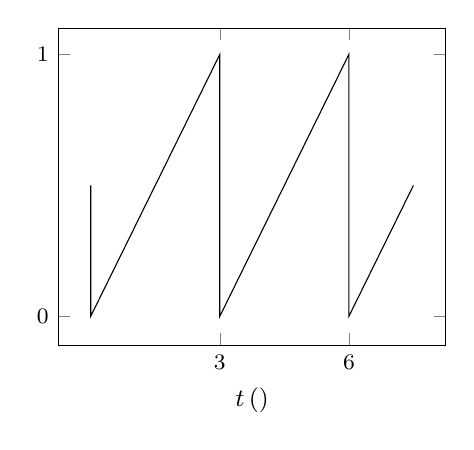
\begin{tikzpicture}
\begin{axis}[small,xlabel={$t\,(\second)$},ylabel style={rotate=-90},xtick={3,6},xticklabels={$3$,$6$},ytick={0,1},yticklabels={$0$,$1$},ymax=1.1]
\addplot[] plot coordinates {(0,0.5)(0,0)  (3,1)  (3,0) (6,1) (6,0) (7.5,0.5)};
\end{axis}
\end{tikzpicture}
\caption*{(الف) دندان موج۔}
\end{subfigure}%
\begin{subfigure}{0.5\textwidth}
\centering
\includegraphics{figFourierSawTooth2}
\caption*{(ب) دو ہارمونی ارکان شامل کئے گئے ہیں۔}
\end{subfigure}
\begin{subfigure}{0.5\textwidth}
\centering
\includegraphics{figFourierSawTooth5}
\caption*{(پ) پانچ ہارمونی ارکان شامل کئے گئے ہیں۔}
\end{subfigure}%
\begin{subfigure}{0.5\textwidth}
\centering
\includegraphics{figFourierSawTooth50}
\caption*{(ت) پچاس ہارمونی ارکان شامل کئے گئے ہیں۔}
\end{subfigure}%
\caption{مثال \حوالہ{مثال_فوریئر_دندان_موج_الف} کی دندان موج۔}
\label{شکل_فوریئر_دندان_موج_الف}
\end{figure}

حل:شکل میں دکھائی گئی موج \عددی{(0,0)} سے \عددی{(3,1)} تک بالکل سیدھی لکیر کی مانند ہے جس کی ڈھلوان 
\begin{align*}
\text{ڈھلوان}=\frac{y_2-y_1}{x_2-x_1}=\frac{1-0}{3-0}=\frac{1}{3}
\end{align*}
ہے لہٰذا اس سیدھے حصے کی مساوات درج ذیل لکھی جا سکتی ہے جہاں لکیر پر کسی بھی نقطے کے کارتیسی محدد مساوات میں پر کرنے سے \عددی{c} کی قیمت حاصل کی جا سکتی ہے۔
\begin{align*}
y=\frac{x}{3}+c
\end{align*}
ہم درج بالا میں \عددی{(0,0)} پر کرتے ہوئے
\begin{align*}
0=\frac{0}{3}+c
\end{align*}
 \عددی{c=0} حاصل کرتے ہیں لہٰذا سیدھی حصے کی مساوات \عددی{y=\tfrac{x}{3}} یعنی
\begin{align}
f(t)=\frac{t}{3}
\end{align}
ہے جہاں کارتیسی نظام کے \عددی{x} محور پر \عددی{t} اور \عددی{y} محور پر \عددی{f(t)} پر کئے گئے ہیں۔

مساوات \حوالہ{مساوات_فوریئر_عددی_سر_ت} سے فوریئر تسلسل کے عددی سر حاصل کرتے ہیں۔
\begin{align*}
a_0&=\frac{1}{T_0}\int_0^{T_0} f(t) \dif t\\
&=\frac{1}{3}\int_0^3 \frac{t}{3} \dif t\\
&=\left. \frac{1}{3} \frac{t^2}{6} \right|_0^3\\
&=\frac{1}{2}
\end{align*}
چونکہ \عددی{a_0} تفاعل کی اوسط قیمت کے برابر ہے لہٰذا یہی جواب تکون کے رقبے \عددی{\tfrac{1}{2}\times 3\times 1=\tfrac{3}{2}} اور قاعدہ \عددی{3} سے حاصل کی جا سکتی ہے یعنی
\begin{align*}
\text{اوسط}&=\frac{\text{رقبہ}}{\text{قاعدہ}}=\frac{\frac{3}{2}}{3}=\frac{1}{2}
\end{align*}
عددی سر \عددی{a_m} حاصل کرتے ہیں۔
\begin{align*}
a_m&=\frac{2}{T_0}\int_0^{T_0} f(t)\cos (m\omega_0 t) \dif t\\
&=\frac{2}{3}\int_0^3 \frac{t}{3} \cos (m \frac{2\pi}{3} t) \dif t\\
&=\left. \frac{2}{9}t \frac{\sin(\frac{2\pi}{3}mt)}{\frac{2\pi}{3}m}+\frac{2}{9}\frac{\cos(\frac{2\pi}{3}mt)}{\left(\frac{2\pi}{3}m\right)^2}\right|_0^3\\
&=0
\end{align*}
اس کا مطلب ہے کہ دندان موج کی فوریئر تسلسل میں کوئی کوسائن تفاعل نہیں پایا جاتا۔

عددی سر \عددی{b_m} حاصل کرتے ہیں۔
\begin{align*}
b_m&=\frac{2}{T_0}\int_0^{T_0} f(t)\sin(m\omega_0 t) \dif t\\
&=\frac{2}{3}\int_0^3 \frac{t}{3}\sin (m\frac{2\pi}{3} t) \dif t\\
&=\left.-\frac{2}{9}t\frac{\cos(\frac{2\pi}{3}mt)}{\frac{2\pi}{3}m}+\frac{2}{9}\frac{\sin(\frac{2\pi}{3}mt)}{\left(\frac{2\pi}{3}m\right)^2}\right|_0^3\\
&=-\frac{1}{m\pi}
\end{align*}
یوں \عددی{m=1,2,3,\cdots} پر کرتے ہوئے عددی سر حاصل ہوتے ہیں یعنی
\begin{align*}
b_1&=-\frac{1}{\pi}\\
b_2&=-\frac{1}{2\pi}\\
b_3&=-\frac{1}{3\pi}\\
&\vdots
\end{align*}
لہٰذا فوریئر تسلسل درج ذیل لکھی جائے گی۔
\begin{align}\label{مساوات_فوریئر_دندان_موج}
f(t)=\frac{1}{2}-\frac{1}{\pi}\left[\sin \omega_0 t+\frac{1}{2} \sin (2\omega_0 t) +\frac{1}{3} \sin (3\omega_0 t)+\cdots\right]
\end{align}
شکل \حوالہ{شکل_فوریئر_دندان_موج_الف}-ب میں  مساوات \حوالہ{مساوات_فوریئر_دندان_موج} کو \عددی{m=2} تک استعمال کرتے ہوئے خط کھینچا گیا ہے۔شکل-پ میں پانچ ہارمونی ارکان استعمال کئے گئے ہیں جبکہ شکل-ت میں پچاس ہارمونی ارکان استعمال کئے گئے ہیں۔آپ دیکھ سکتے ہیں کہ ارکان بڑھانے سے اصل موج کے قریب تر خط حاصل کیا جا سکتا ہے۔
\انتہا{مثال}
%========================
\ابتدا{مثال}\شناخت{مثال_فوریئر_مستطیل_موج}
آئیں شکل \حوالہ{شکل_فوریئر_مستطیل_موج_الف}-الف  میں دکھائے گئے  دوری مستطیل موج کا فوریئر تسلسل حاصل کریں جس میں دوری عرصے کو \عددی{T} لکھا گیا ہے۔
\begin{figure}
\centering
\begin{subfigure}{0.5\textwidth}
\centering
\begin{tikzpicture}
\begin{axis}[small,xlabel={$t$},ylabel style={rotate=-90},xtick={-2,-1,0,1,2,3},xticklabels={$-\frac{T}{2}$,$-\frac{T}{4}$,$0$,$\frac{T}{4}$,$\frac{T}{2}$,$\frac{3T}{4}$},ytick={-1,1},yticklabels={$-V_0$,$V_0$}]
\addplot[] plot coordinates {(-4,1) (-3,1) (-3,-1) (-1,-1) (-1,1) (1,1) (1,-1) (3,-1) (3,1)(4,1)};
\end{axis}
\end{tikzpicture}
\caption*{(الف) مستطیل موج۔}
\end{subfigure}%
\begin{subfigure}{0.5\textwidth}
\centering
\includegraphics{figFourierSquareWave5}
\caption*{(ب) ایک، تین اور پانچ ہارمونی ارکان کا مجموعہ یعنی \عددی{m=5} ہے۔}
\end{subfigure}
\begin{subfigure}{0.5\textwidth}
\centering
\includegraphics{figFourierSquareWave10}
\caption*{((پ) \عددی{m=9} تک ارکان کا مجموعہ۔}
\end{subfigure}%
\begin{subfigure}{0.5\textwidth}
\centering
\includegraphics{figFourierSquareWave50}
\caption*{(ت) \عددی{m=49} تک ارکان کا مجموعہ۔}
\end{subfigure}
\caption{مثال \حوالہ{مثال_فوریئر_مستطیل_موج} کی مستطیل موج۔}
\label{شکل_فوریئر_مستطیل_موج_الف}
\end{figure}

حل:افقی محور کے دونوں اطراف برابر موج پائی جاتی ہے لہٰذا اس کی اوسط قیمت صفر ہو گی اور یوں \عددی{a_0=0} ہو گا۔آئیں یہی جواب مساوات \حوالہ{مساوات_فوریئر_عددی_سر_ت} سے حاصل کریں۔اس مرتبہ ہم دوری عرصے کو \عددی{-\tfrac{T}{2} \le t \le \tfrac{T}{2}} لیتے ہیں۔شکل کو دیکھ معلوم ہوتا ہے کہ \عددی{-\tfrac{T}{4} \le t \le \tfrac{T}{4}} تفاعل کی قیمت \عددی{V_0} ہے جبکہ
 \عددی{-\frac{T}{2}\le t \le -\tfrac{T}{4}} اور \عددی{\tfrac{T}{4} \le t \le \tfrac{T}{2}} پر تفاعل کی قیمت \عددی{-V_0} ہے۔
\begin{align*}
a_0&=\frac{1}{T}\int_0^T f(t) \dif t\\
&=\frac{1}{T} \left(-V_0 \int_{-\frac{T}{2}}^{-\frac{T}{4}} \dif t+V_0\int_{-\frac{T}{4}}^{\frac{T}{4}}\dif t -V_0\int_{\frac{T}{4}}^{\frac{T}{2}} \dif t\right)\\
&=\frac{1}{T}\left[-V_0\left(-\frac{T}{4}+\frac{T}{2}\right)+V_0\left(\frac{T}{4}+\frac{T}{4}\right)-V_0\left(\frac{T}{2}-\frac{T}{4}\right)\right]\\
&=0
\end{align*}
کوسائن کے عددی سر \عددی{a_m} کو مساوات \حوالہ{مساوات_فوریئر_عددی_سر_ت} کی مدد سے حاصل کرتے ہیں۔مستقل \عددی{V_0} کو تکمل کے باہر لکھا گیا ہے۔
\begin{align*}
a_m&=\frac{2}{T}\int_0^T f(t)\cos(m\omega_0 t) \dif t\\
&=-\frac{2}{T}V_0\int_{-\frac{T}{2}}^{-\frac{T}{4}} \cos (\frac{2\pi m}{T} t) \dif t+\frac{2}{T}V_0\int_{-\frac{T}{4}}^{\frac{T}{4}} \cos (\frac{2\pi m}{T} t) \dif t-\frac{2}{T}V_0\int_{\frac{T}{4}}^{\frac{T}{2}} \cos (\frac{2\pi m}{T} t) \dif t\\
&=-\frac{2V_0}{T}\left.\frac{\sin (\frac{2\pi m}{T} t)}{\frac{2\pi m}{T}}\right|_{-\frac{T}{2}}^{-\frac{T}{4}}+\frac{2V_0}{T}\left.\frac{\sin (\frac{2\pi m}{T} t)}{\frac{2\pi m}{T}}\right|_{-\frac{T}{4}}^{\frac{T}{4}}-\frac{2V_0}{T}\left.\frac{\sin (\frac{2\pi m}{T} t)}{\frac{2\pi m}{T}}\right|_{\frac{T}{4}}^{\frac{T}{2}}\\
&=\frac{4V_0}{m\pi} \sin(\frac{m\pi}{2})
\end{align*}
اس سے درج ذیل عددی سر لکھے جا سکتے ہیں۔
\begin{align*}
a_1&=\frac{4V_0}{1\pi} \sin(\frac{1\pi}{2})=\frac{4V_0}{\pi}\\
a_2&=\frac{4V_0}{2\pi} \sin(\frac{2\pi}{2})=0\\
a_3&=\frac{4V_0}{3\pi} \sin(\frac{3\pi}{2})=-\frac{4V_0}{3\pi}\\
a_4&=\frac{4V_0}{4\pi} \sin(\frac{4\pi}{2})=0\\
a_5&=\frac{4V_0}{5\pi} \sin(\frac{5\pi}{2})=\frac{4V_0}{5\pi}\\
&\vdots
\end{align*}
سائن کے عددی سر \عددی{b_m} کو مساوات \حوالہ{مساوات_فوریئر_عددی_سر_ت} کی مدد سے حاصل کرتے ہیں۔مستقل \عددی{V_0} کو تکمل کے باہر لکھا گیا ہے۔
\begin{align*}
b_m&=\frac{2}{T}\int_0^T f(t)\sin(m\omega_0 t) \dif t\\
&=-\frac{2}{T}V_0\int_{-\frac{T}{2}}^{-\frac{T}{4}} \sin (\frac{2\pi m}{T} t) \dif t+\frac{2}{T}V_0\int_{-\frac{T}{4}}^{\frac{T}{4}} \sin (\frac{2\pi m}{T} t) \dif t-\frac{2}{T}V_0\int_{\frac{T}{4}}^{\frac{T}{2}} \sin (\frac{2\pi m}{T} t) \dif t\\
&=\frac{2V_0}{T}\left.\frac{\cos (\frac{2\pi m}{T} t)}{\frac{2\pi m}{T}}\right|_{-\frac{T}{2}}^{-\frac{T}{4}}-\frac{2V_0}{T}\left.\frac{\cos (\frac{2\pi m}{T} t)}{\frac{2\pi m}{T}}\right|_{-\frac{T}{4}}^{\frac{T}{4}}+\frac{2V_0}{T}\left.\frac{\cos (\frac{2\pi m}{T} t)}{\frac{2\pi m}{T}}\right|_{\frac{T}{4}}^{\frac{T}{2}}\\
&=0
\end{align*}
اس معلومات کو استعمال کرتے ہوئے مستطیل موج کی فوریئر مساوات لکھتے ہیں۔
\begin{align}\label{مساوات_فوریئر_مستطیل_موج}
f(t)=\frac{4V_0}{\pi}\left[\cos (\omega_0 t)-\frac{1}{3}\cos(3\omega_0 t)+\frac{1}{5}\cos(5\omega_0 t)-\frac{1}{7}\cos(7\omega_0 t)+\cdots\right]
\end{align}
مختلف تعداد میں فوریئر تسلسل کے ارکان شامل کرتے ہوئے تفاعل کو شکل \حوالہ{شکل_فوریئر_مستطیل_موج_الف}-ب تا شکل \حوالہ{شکل_فوریئر_مستطیل_موج_الف}-ت میں دکھایا گیا ہے۔
\انتہا{مثال}
%=======================

مثال \حوالہ{مثال_فوریئر_مستطیل_موج} میں مستطیل موج کی فوریئر تسلسل  حاصل کی گئی۔آئیں تسلسل کے ایک رکن سے شروع کرتے ہوئے دیکھیں کہ اس میں مزید ارکان شامل کرتے ہوئے مستطیل موج کیسے حاصل ہوتی ہے۔شکل \حوالہ{شکل_فوریئر_ابھرتا_مستطیل}-الف میں  مساوات \حوالہ{مساوات_فوریئر_مستطیل_موج} کا پہلا ہارمونی رکن \عددی{\tfrac{4V_0}{\pi}\cos\omega_0 t} اور تیسرا ہارمونی رکن \عددی{-\frac{4V_0}{3\pi}\cos(3\omega_0t)} ہلکی سیاہی میں دکھائے گئے ہیں۔دونوں سائن نما صورت رکھتے ہیں جس کا مستطیل سے دور دور تک کوئی واسطہ نہیں ہے۔اسی شکل میں دونوں کے مجموعے کو گہری سیاہی میں دکھایا گیا ہے۔آپ دیکھ سکتے ہیں کہ دو سائن نما امواج مل کر ایسی شکل بناتے ہیں جو مستطیل زیادہ اور سائن نما کم نظر آتا ہے۔مستطیل موج کی چوٹی \عددی{V_0} ہے جبکہ پہلے ہارمونی رکن کی چوٹی \عددی{\tfrac{4V_0}{\pi}=1.27V_0} ہے۔تیسرا ہارمونی رکن اس چوٹی کو نیچے کھینچتا ہے۔اسی طرح مستطیل موج \عددی{\mp \tfrac{T}{4}} پر یکدم قیمت تبدیل کرتی ہے جبکہ پہلا ہارمونی جزو نہایت صبروتحمل کے ساتھ منفی چوٹی سے مثبت چوٹی اور مثبت چوٹی سے منفی چوٹی پہنچتی ہے۔ یہاں بھی تیسرا ہارمونی رکن پہلے رکن کے اطراف کو کھینچ کر ان کی ڈھلوان بڑھاتی ہے۔

\begin{figure}
\centering
\begin{subfigure}{0.5\textwidth}
\centering
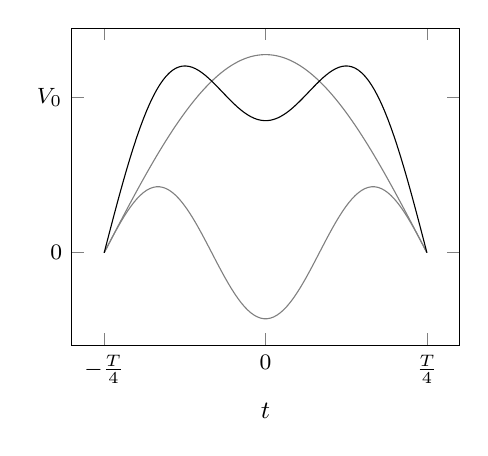
\begin{tikzpicture}
\begin{axis}[small,xlabel={$t$},ylabel style={rotate=-90},xtick={-2,-1,0,1,2},xticklabels={$-\frac{T}{2}$,$-\frac{T}{4}$,$0$,$\frac{T}{4}$,$\frac{T}{2}$},ytick={0,1},yticklabels={$0$,$V_0$}]
\addplot[gray,domain=-1:1,samples=100]{4/pi*cos(90*x)};
\addplot[gray,domain=-1:1,samples=100]{-4/(3*pi)*cos(3*90*x)};
\addplot[black,domain=-1:1,samples=100]{4/pi*cos(90*x)-4/(3*pi)*cos(3*90*x)};
\end{axis}
\end{tikzpicture}
\caption*{(الف) پہلا اور تیسرا ہارمونی رکن مل کر مستطیل صورت بنانے کی کوشش کرتے ہیں۔}
\end{subfigure}%
\begin{subfigure}{0.5\textwidth}
\centering
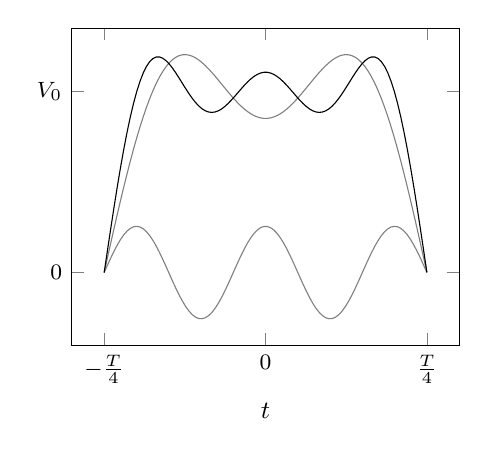
\begin{tikzpicture}
\begin{axis}[small,xlabel={$t$},ylabel style={rotate=-90},xtick={-2,-1,0,1,2},xticklabels={$-\frac{T}{2}$,$-\frac{T}{4}$,$0$,$\frac{T}{4}$,$\frac{T}{2}$},ytick={0,1},yticklabels={$0$,$V_0$}]
\addplot[gray,domain=-1:1,samples=100]{4/pi*cos(90*x)-4/(3*pi)*cos(3*90*x)};
\addplot[gray,domain=-1:1,samples=100]{4/(5*pi)*cos(5*90*x)};
\addplot[black,domain=-1:1,samples=100]{4/pi*cos(90*x)-4/(3*pi)*cos(3*90*x)+4/(5*pi)*cos(5*90*x)};
\end{axis}
\end{tikzpicture}
\caption*{(ب) پہلے،تیسرا اور پانچواں ہارمونی ارکان مل کر مستطیل شکل بناتے ہیں۔}
\end{subfigure}
\caption{بتدریج زیادہ ارکان شامل کرتے ہوئے مستطیل موج کی صورت ابھرتے ہوئے دیکھتے ہیں۔}
\label{شکل_فوریئر_ابھرتا_مستطیل}
\end{figure}

شکل \حوالہ{شکل_فوریئر_ابھرتا_مستطیل}-الف میں تیسرا رکن زیادہ جزبات میں آ کر پہلی رکن کی چوٹی ضرورت سے زیادہ نیچے کھینچ  دیتا ہے۔شکل-ب میں پہلے اور تیسرے ارکان سے حاصل موج کو ہلکی سیاہی میں دکھایا گیا ہے۔ساتھ ہی ساتھ پانچویں رکن کو بھی ہلکی سیاہی میں دکھایا گیا ہے۔ان کے مجموعے کو گہری سیاہی میں دکھایا گیا ہے۔آپ دیکھ سکتے ہیں پانچواں رکن ضرورت سے زیادہ نیچے کھینچی گئی چوٹی کو معمولی اٹھاتا ہے تا کہ یہ \عددی{V_0} کے قریب ہو جائے۔اسی طرح یہ رکن بھی موج کے اطراف کی ڈھلوان بڑھاتا ہے۔فوریئر تسلسل کے بقایا ارکان بھی اسی طرح مدد کرتے ہوئے اطراف کو زیادہ عمودی اور چوٹی کو بالکل چپٹی بنانے میں مدد دیتے ہیں حتٰی کہ ہمیں بالکل مستطیل موج نظر آتی ہے۔

شکل \حوالہ{شکل_فوریئر_مستطیل_موج_الف}-ب، پ اور ت میں آپ دیکھتے ہیں کہ فوریئر تسلسل سے حاصل موج \عددی{\mp \tfrac{T}{4}} پر درکار قیمت سے تجاوز کرتے ہوئے آگے نکل جاتی ہے۔تسلسل میں ارکان کی تعداد بڑھانے سے ان تجاوزات کا خاتمہ نہیں ہوتا۔
%======================
\ابتدا{مشق}
شکل \حوالہ{شکل_فوریئر_مستطیل_موج_الف}-الف میں عددی سر حاصل کرتے ہوئے تکملات کو \عددی{-\tfrac{T}{4}\le t\le \tfrac{3T}{4}} پر حاصل کرتے ہوئے فوریئر تسلسل حاصل کریں۔

جواب:عددی سر حاصل کرتے ہوئے دوری موج کے کسی بھی حصے پر مسلسل ایک دوری عرصے پر تکمل حاصل کیا جا سکتا ہے۔جوابات میں کوئی فرق نہیں پایا جاتا۔
\انتہا{مشق}
%=======================
\ابتدا{مشق}\شناخت{مشق_فوریئر_مشق_مستطیل}
شکل \حوالہ{شکل_فوریئر_مشق_مستطیل}-الف میں دکھائے گئے مستطیل موج کی فوریئر تسلسل حاصل کریں۔
\begin{figure}
\centering
\begin{subfigure}{0.5\textwidth}
\centering
\begin{tikzpicture}
\begin{axis}[small,xlabel={$t$},ylabel style={rotate=-90},xtick={0,1,2},xticklabels={$0$,$\frac{T}{2}$,$T$},ytick={-1,0,1},yticklabels={$-V_0$,$0$,$V_0$}]
\addplot[] plot coordinates{(-0.25,-1) (0,-1) (0,1) (1,1) (1,-1) (2,-1) (2,1) (3,1) (3,-1) (3.25,-1)};
\end{axis}
\end{tikzpicture}
\caption*{(الف) مستطیل موج۔}
\end{subfigure}%
\begin{subfigure}{0.5\textwidth}
\centering
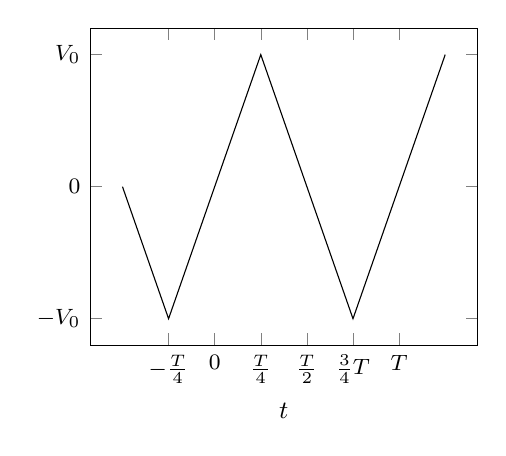
\begin{tikzpicture}
\begin{axis}[small,xlabel={$t$},ylabel style={rotate=-90},xtick={-1,0,1,2,3,4},xticklabels={$-\frac{T}{4}$,$0$,$\frac{T}{4}$,$\frac{T}{2}$,$\frac{3}{4}T$,$T$},ytick={-1,0,1},yticklabels={$-V_0$,$0$,$V_0$}]
\addplot[] plot coordinates{(-2,0)(-1,-1) (1,1) (3,-1) (5,1) };
\end{axis}
\end{tikzpicture}
\caption*{(ب) تکونی موج۔}
\end{subfigure}
\caption{مشق \حوالہ{مشق_فوریئر_مشق_مستطیل} اور مشق \حوالہ{مشق_فوریئر_مشق_تکونی} کے امواج۔}
\label{شکل_فوریئر_مشق_مستطیل}
\end{figure}

جواب:
$f(t)=\frac{4V}{\pi}\left[\sin \omega_0 t+\frac{1}{3}\sin(3\omega_0 t)+\frac{1}{5}\sin(5\omega_0 t)+\cdots\right]$
\انتہا{مشق}
%=======================
\ابتدا{مشق}\شناخت{مشق_فوریئر_مشق_تکونی}
شکل \حوالہ{شکل_فوریئر_مشق_مستطیل}-ب میں دکھائے گئے تکونی موج کی فوریئر تسلسل حاصل کریں۔پہلے \عددی{-\tfrac{T}{4} \le t \le \tfrac{T}{4}} اور 
\عددی{\tfrac{T}{4} \le t \le\tfrac{3T}{4}} سیدھے حصوں کے مساوات حاصل کریں۔

حل:\عددی{f_1(t)=\tfrac{4V_0}{T}t}، \عددی{f_2(t)=2V_0(1-2\tfrac{t}{T})}، \\
$f(t)=\tfrac{8V_0}{\pi^2}\left[\sin(\omega_0 t)-\tfrac{1}{3^2}\sin(3\omega_0 t)+\tfrac{1}{5^2}\sin(5\omega_0 t)-\cdots\right]$
\انتہا{مشق}
%=========================
\ابتدا{مشق}\شناخت{مشق_فوریئر_مختلف_تفاعل_مشق}
شکل \حوالہ{شکل_فوریئر_مختلف_تفاعل_مشق} میں دیے تفاعل کی فوریئر تسلسل حاصل کریں۔
\begin{figure}
\centering
\begin{tikzpicture}
\begin{axis}[xtick={0,1,2,3,4},xticklabels={$0$,$1$,$2$,$3$,$4$},ytick={0,1,2},yticklabels={$0$,$1$,$2$}]
\addplot[] plot coordinates {(0,0) (1,0) (1,1) (2,1) (2,2) (3,2) (3,0) (4,0) (4,1) (5,1) (5,2) (6,2) (6,0)};
\end{axis}
\end{tikzpicture}
\caption{مشق \حوالہ{مشق_فوریئر_مختلف_تفاعل_مشق} کا تفاعل۔}
\label{شکل_فوریئر_مختلف_تفاعل_مشق}
\end{figure}

جواب:
\begin{align*}
1-\tfrac{3}{\pi}\left[\sin \omega_0 t+\tfrac{1}{2}\sin (2\omega_0 t)+\tfrac{1}{4}\sin(4\omega_0 t)+\tfrac{1}{5}\sin(5\omega_0 t)+\tfrac{1}{7}\sin(7\omega_0 t)+\cdots\right]
\end{align*}
\انتہا{مشق}
%======================================================================

فوریئر تسلسل کے \عددی{m} ہارمونی کو درج ذیل لکھا جا سکتا ہے
\begin{align*}
a_m\cos(m\omega_0 t)+b_m\sin(m\omega_0 t)=D_m\cos(m\omega_0 t+\theta_m)
\end{align*} 
جہاں
\begin{align}\label{مساوات_فوریئر_رداس_زاویہ}
D_m&=\sqrt{a_m^2+b_m^2}\\
\theta_m&=\tan^{-1}\frac{b_m}{a_m}
\end{align}
 ہیں۔یوں  \اصطلاح{تکونیاتی فوریئر تسلسل}\فرہنگ{فوریئر تسلسل!تکونیاتی} کی دوسری صورت درج ذیل لکھی جا سکتی ہے۔
\begin{gather}
\begin{aligned}\label{مساوات_فوریئر_تسلسل_صورت_ب}
f(t)&=a_0+D_1\cos(\omega_0 t+\theta_1)+D_2\cos(2\omega_0 t+\theta_2)+\cdots\\
&=a_0+\sum_{n=1}^{\infty} D_n \cos(n\omega_0 t +\theta_n)
\end{aligned}
\end{gather}
چونکہ \عددی{\cos x=\tfrac{e^{jx}+e^{-jx}}{2}} لکھا جا سکتا ہے لہٰذا مساوات \حوالہ{مساوات_فوریئر_تسلسل_صورت_ب} کو درج ذیل لکھا جا سکتا ہے۔
\begin{align*}
f(t)&=a_0+\sum_{n=1}^{\infty} D_n \cos(n\omega_0 t +\theta_n)\\
&=a_0+\sum_{n=1}^{\infty} D_n \frac{e^{j(n\omega_0 t+\theta_n)}+e^{-j(n\omega_0 t+\theta_n)}}{2}\\
&=a_0+\sum_{n=1}^{\infty} \frac{D_n e^{j\theta_n}}{2} e^{jn\omega_0 t}+\sum_{n=1}^{\infty} \frac{D_n e^{-j\theta_n}}{2}e^{-jn\omega_0 t}
\end{align*}
مساوات \حوالہ{مساوات_فوریئر_رداس_زاویہ} کے تحت \عددی{D_m} حقیقی مقدار ہے لہٰذا درج بالا مساوات میں \عددی{\tfrac{D_ne^{j\theta_n}}{2}} اور
 \عددی{\tfrac{D_ne^{-j\theta_n}}{2}} آپس میں جوڑی دار مخلوط ہیں۔ یوں \عددی{\tfrac{D_ne^{j\theta_n}}{2}=\kx{d_n}} لکھتے ہوئے
 \عددی{\tfrac{D_ne^{-j\theta_n}}{2}=\kx{d}^*_n} لکھا جائے گا لہٰذا درج بالا کو درج ذیل لکھ سکتے ہیں۔
\begin{align}\label{مساوات_فوریئر_تسلسل_پ}
f(t)&=a_0+\sum_{n=1}^{\infty} \kx{d}_n e^{jn\omega_0 t}+\sum_{n=1}^{\infty} \kx{d}^*_n e^{-jn\omega_0 t}
\end{align}
دونوں مجموعوں کو پھیلا کر لکھتے ہیں
\begin{multline*}
\sum_{n=1}^{\infty} \kx{d}_n e^{jn\omega_0 t}+\sum_{n=1}^{\infty} \kx{d}^*_n e^{-jn\omega_0 t}\\
=\kx{d}_1 e^{j1\omega_0 t}+\kx{d}_2 e^{j2\omega_0 t}+\cdots +\kx{d}^*_1 e^{-j1\omega_0 t}+\kx{d}^*_2 e^{-j2\omega_0 t}+\cdots \\
=\cdots+\kx{d}^*_2 e^{-j2\omega_0 t}+\kx{d}^*_1 e^{-j1\omega_0 t}+\kx{d}_1 e^{j1\omega_0 t}+\kx{d}_2 e^{j2\omega_0 t}+\cdots
\end{multline*}
جہاں  آخری قدم پر \عددی{e} کی طاقت کے لہٰذا سے ترتیب دیا گیا ہے۔آپ دیکھ سکتے ہیں کہ \عددی{n=0} کے علاوہ درج بالا تسلسل کی وسعت منفی لامتناہی سے مثبت لامتناہی تک ہے۔اس تسلسل کو درج ذیل لکھا جا سکتا ہے جہاں عددی سر کو \عددی{\kx{c}_n} کہا گیا ہے۔
\begin{align*}
\sum_{n=1}^{\infty} \kx{d}_n e^{jn\omega_0 t}+\sum_{n=1}^{\infty} \kx{d}^*_n e^{-jn\omega_0 t}=\sum_{\substack{n=-\infty\\ n \ne 0 \hfill}}^{\infty} \kx{c}_n e^{jn\omega_0 t}
\end{align*}
یوں مساوات \حوالہ{مساوات_فوریئر_تسلسل_پ} سے فوریئر تسلسل کی تیسری صورت یعنی \اصطلاح{قوت نمائی فوریئر تسلسل}\فرہنگ{قوت نمائی فوریئر تسلسل}\فرہنگ{فوریئر تسلسل!قوت نمائی}\حاشیہب{exponential Fourier series}\فرہنگ{Fourier series!exponential} حاصل ہوتی ہے جہاں تسلسل کے عددی سر \عددی{\kx{c}_n} مخلوط مقدار ہیں۔
\begin{gather}
\begin{aligned}\label{مساوات_فوریئر_تسلسل_صورت_ت}
f(t)&=a_0+\sum_{\substack{n=-\infty\\ n \ne 0 \hfill}}^{\infty} \kx{c}_n e^{jn\omega_0 t}\\
&=\sum_{n=-\infty}^{\infty} \kx{c}_n e^{jn\omega_0 t}
\end{aligned}
\end{gather}
مجموعے میں \عددی{n=0} کا رکن شامل کرتے ہوئے بیرونی رکن \عددی{a_0} کو مجموعے میں ضم کیا گیا ہے۔

تینوں طرز کے فوریئر تسلسل کے عددی سر کا تعلق درج ذیل ہے۔
\begin{align}
D_n\phase{\theta_n}=2\kx{c}_n=a_n-jb_n
\end{align}

قوت نمائی فوریئر تسلسل کا عددی سر \عددی{\kx{c}_m} حاصل کرنے کی خاطر مساوات \حوالہ{مساوات_فوریئر_تسلسل_صورت_ت} کے دونوں اطراف کو \عددی{e^{-jm\omega_0 t}} سے ضرب دیتے ہوئے \عددی{0 \le t \le T_0} پر ان کا تکمل حاصل کیا جاتا ہے۔
\begin{align}\label{مساوات_فوریئر_عددی_سر_قوت_نما_الف}
\int_0^{T_0}f(t)e^{-jm\omega_0 t} \dif t=\sum_{n=-\infty}^{\infty} \int_0^{T_0}\kx{c}_ne^{j(n-m)\omega_0 t} \dif t
\end{align}
اگر \عددی{n\ne m} ہو تب
\begin{align*}
\int_0^{T_0} \kx{c}_ne^{j(n-m)\omega_0 t} \dif t&=\left. \frac{\kx{c}_ne^{j(n-m)\omega_0 t}}{j(n-m)\omega_0}\right|_0^{T_0}\\
&=\frac{\kx{c}_n \left[e^{j(n-m)2\pi}-e^{0}\right]}{j(n-m)\omega_0}\\
&=0
\end{align*}
ملتا ہے جہاں آخری قدم پر \عددی{e^{j(n-m)2\pi}=\cos[(n-m)2\pi]+j\sin[(n-m)2\pi]=1} اور \عددی{e^0=1} کا استعمال کیا گیا ہے۔اس کے برعکس \عددی{n=m} کی صورت میں \عددی{\kx{c}_n} کو \عددی{\kx{c}_m} لکھا جا سکتا ہے اور
\begin{align*}
\int_0^{T_0} \kx{c}_m \dif t=T_0 \kx{c}_m
\end{align*}
ہو گا لہٰذا مساوات \حوالہ{مساوات_فوریئر_عددی_سر_قوت_نما_الف} کو درج ذیل لکھا جا سکتا ہے۔
\begin{align}\label{مساوات_فوریئر_عددی_سر_قوت_نما_ب}
\kx{c}_m=\frac{1}{T_0} \int_0^{T_0} f(t) e^{-jm\omega_0 t} \dif t
\end{align}
%======================================================================
\ابتدا{مثال}\شناخت{مثال_فوریئر_دندان_دوبارہ}
ہم شکل \حوالہ{شکل_فوریئر_مشق_مستطیل}-الف کے مستطیل تفاعل کا تکونیاتی فوریئر تسلسل حاصل کر چکے ہیں۔آئیں اس کی قوت نمائی فوریئر تسلسل حاصل کریں۔تفاعل کو شکل \حوالہ{شکل_فوریئر_دندان_دوبارہ} میں دوبارہ دکھایا گیا ہے۔
\begin{figure}
\centering
\begin{tikzpicture}
\begin{axis}[small,xlabel={$t$},ylabel style={rotate=-90},xtick={0,1,2},xticklabels={$0$,$\frac{T}{2}$,$T$},ytick={-1,0,1},yticklabels={$-V_0$,$0$,$V_0$}]
\addplot[] plot coordinates{(-0.25,-1) (0,-1) (0,1) (1,1) (1,-1) (2,-1) (2,1) (3,1) (3,-1) (3.25,-1)};
\end{axis}
\end{tikzpicture}
\caption{مثال \حوالہ{مثال_فوریئر_دندان_دوبارہ} کا تفاعل۔}
\label{شکل_فوریئر_دندان_دوبارہ}
\end{figure}%

حل: مساوات \حوالہ{مساوات_فوریئر_عددی_سر_قوت_نما_ب} استعمال کرتے ہوئے  \عددی{c\kx{c}_0} حاصل کرتے ہیں۔
\begin{align*}
\kx{c}_0&=\frac{1}{T}\int_0^{T} f(t) \dif t\\
&=\frac{1}{T}\int_0^{\frac{T}{2}} V_0 \dif t+\frac{1}{T}\int_{\frac{T}{2}}^{T}(-V_0)\dif t\\
&=0
\end{align*}
اسی طرح \عددی{\kx{c}_m} حاصل کرتے ہیں۔
\begin{align*}
\kx{c}_m&=\frac{1}{T} \int_0^{T} f(t) e^{-jm\omega_0 t} \dif t\\
&=\frac{V_0}{T}\int_0^{\frac{T}{2}} e^{-jm\omega_0 t} \dif t-\frac{V_0}{T}\int_{\frac{T}{2}}^T e^{-jm\omega_0 t} \dif t\\
&=\left. \frac{V_0 e^{-jm\omega_0 t}}{-jm\omega_0 T}\right|_{0}^{\frac{T}{2}}-\left. \frac{V_0 e^{-jm\omega_0 t}}{-jm\omega_0 T}\right|_{\frac{T}{2}}^{T}\\
&=\frac{jV_0}{m\pi}(\cos m\pi -1)\quad \substack{-\infty \le m \le \infty\\ m \ne 0}
\end{align*}
جس سے درج ذیل لکھا جا سکتا ہے۔
\begin{align*}
\kx{c}_1&=\kx{c}^*_1=-\frac{j2V_0}{\pi}\\
\kx{c}_2&=\kx{c}^*_2=0\\
\kx{c}_3&=\kx{c}^*_3=-\frac{j2V_0}{3\pi}\\
\kx{c}_4&=\kx{c}^*_4=0\\
\kx{c}_5&=\kx{c}^*_5=-\frac{j2V_0}{5\pi}
\end{align*}
یوں شکل میں دیے مستطیل تفاعل کی فوریئر تسلسل درج ذیل ہو گی۔
\begin{align} \label{مساوات_فوریئر_مستطیل_دوسرا_جواب}
f(t)&=\sum_{\substack{n=-\infty \\ n=\text{طاق}\\ n \ne 0} }^{\infty} -\frac{j2V_0}{n\pi}e^{jn\omega_0 t}
\end{align}
\انتہا{مثال}
%===================================
\ابتدا{مشق}
مساوات \حوالہ{مساوات_فوریئر_مستطیل_دوسرا_جواب} میں \عددی{\kx{c}_ne^{jn\omega_0 t}+\kx{c}^*_ne^{-jn\omega_0t}} اکٹھے کرتے ہوئے مشق \حوالہ{مشق_فوریئر_مشق_مستطیل} میں دیا جواب حاصل کریں۔
\انتہا{مشق}
%======================================
\ابتدا{مشق}\شناخت{مشق_فوریئر_جفت_تفاعل_قوت_نمائی_تسلسل_الف}
شکل \حوالہ{شکل_فوریئر_جفت_تفاعل_قوت_نمائی_تسلسل_الف}-الف میں دیے تفاعل کے قوت نمائی فوریئر تسلسل کے عددی سر معلوم کریں۔
\begin{figure}
\centering
\begin{subfigure}{0.5\textwidth}
\centering
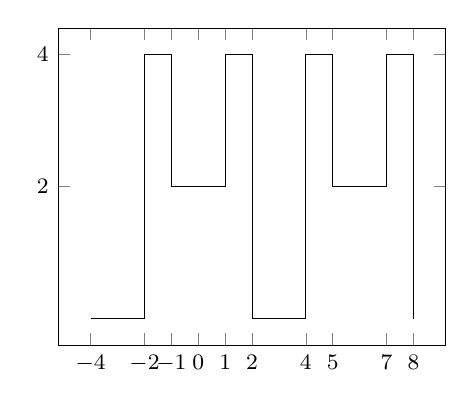
\begin{tikzpicture}
\begin{axis}[small,xtick={-4,-2,-1,0,1,2,4,5,7,8},xticklabels={$-4$,$-2$,$-1$,$0$,$1$,$2$,$4$,$5$,$7$,$8$},ytick={2,4},yticklabels={$2$,$4$}]
\addplot[] plot coordinates { (-4,0) (-2,0) (-2,4) (-1,4) (-1,2) (1,2) (1,4) (2,4) (2,0) (4,0) (4,4) (5,4) (5,2) (7,2) (7,4) (8,4) (8,0)};
\end{axis}
\end{tikzpicture}
\caption*{(الف)}
\end{subfigure}%
\begin{subfigure}{0.5\textwidth}
\centering
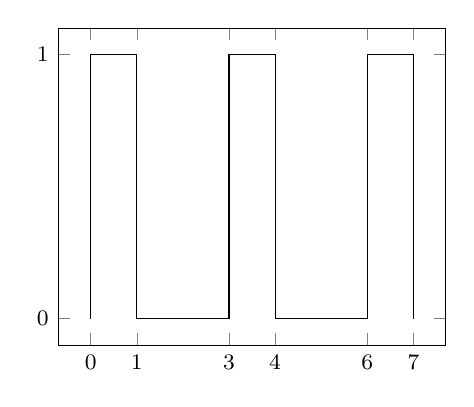
\begin{tikzpicture}
\begin{axis}[small,xtick={0,1,3,4,6,7},xticklabels={$0$,$1$,$3$,$4$,$6$,$7$},ytick={0,1},yticklabels={$0$,$1$}]
\addplot[] plot coordinates { (0,0) (0,1) (1,1) (1,0) (3,0) (3,1) (4,1) (4,0) (6,0) (6,1) (7,1) (7,0) };
\end{axis}
\end{tikzpicture}
\caption*{(ب)}
\end{subfigure}%
\caption{مشق \حوالہ{مشق_فوریئر_جفت_تفاعل_قوت_نمائی_تسلسل_الف} اور مشق \حوالہ{مشق_فوریئر_جفت_تفاعل_قوت_نمائی_تسلسل_ب} کے تفاعل۔}
\label{شکل_فوریئر_جفت_تفاعل_قوت_نمائی_تسلسل_الف}
\end{figure}

جوابات:
\begin{align*}
\kx{c}_0&=\frac{1}{2}\\
\kx{c}_n&=\frac{2}{n\pi}\left[2\sin \frac{2\pi n}{3}-\sin\frac{n\pi}{3}\right]
\end{align*}
\انتہا{مشق}
%================

\ابتدا{مشق}\شناخت{مشق_فوریئر_جفت_تفاعل_قوت_نمائی_تسلسل_ب}
شکل \حوالہ{شکل_فوریئر_جفت_تفاعل_قوت_نمائی_تسلسل_الف}-ب میں دیے تفاعل کے قوت نمائی فوریئر تسلسل کے عددی سر معلوم کریں۔

جوابات:
\begin{align*}
\kx{c}_0&=\frac{1}{3}\\
\kx{c}_n&=\frac{1-e^{-j\frac{2}{3}n\pi}}{j2n\pi}
\end{align*}
\انتہا{مشق}
%======================================================================
\حصہ{تشاکل تفاعل}
آپ نے مختلف تفاعل کے فوریئر تسلسل دیکھے۔ان میں کئی ایسے تھے جن کے یا تمام \عددی{a_m} اور یا تمام \عددی{b_m} صفر کے برابر تھے۔آئیں اس کی وجہ سمجھیں اور تکملات حل کرنے سے پہلے یہ دریافت کرنا سیکھیں کہ آیا فوریئر تسلسل میں \عددی{a_m} اور یا تمام \عددی{b_m} صفر کے برابر ہوں گے۔فوریئر تسلسل کے ارکان کا دارومدار تفاعل کی شکل و صورت پر ہے۔ تین قسم کے تشاکل تفاعل پائے جاتے ہیں۔ان پر باری باری غور کرتے ہیں۔

\جزوحصہ{جفت تفاعل تشاکل}
جفت تفاعل سے مراد ایسا تفاعل ہے جو درج ذیل مساوات پر پورا اترتا ہو۔
\begin{align}
f(t)=f(-t)
\end{align}
جفت  تفاعل عمودی محور کے دونوں اطراف یکساں دکھائی دیتا ہے۔جفت تفاعل کی اہم مثال \عددی{\cos(n\omega_0 t)} ہے۔آپ جانتے ہیں کہ \عددی{\cos(\theta)=\cos(-\theta)} ہوتا ہے لہٰذا یہ جفت تفاعل ہے۔شکل \حوالہ{شکل_فوریئر_مستطیل_موج_الف}-الف بھی جفت تفاعل ہے۔ آئیں جفت تفاعل کے فوریئر تسلسل کے عددی سر حاصل کریں۔

مساوات \حوالہ{مساوات_فوریئر_عددی_سر_ت} میں تکمل کو \عددی{-\tfrac{T_0}{2}\le  t \le \tfrac{T_0}{2}} لیتے ہوئے یہاں دوبارہ پیش کرتے ہیں۔
\begin{gather}
\begin{aligned}\label{مساوات_فوریئر_عددی_سر_جفت}
a_0&=\frac{1}{T_0}\int_{-\frac{T_0}{2}}^{\frac{T_0}{2}}f(t) \dif t\\
a_m&=\frac{2}{T_0}\int_{-\frac{T_0}{2}}^{\frac{T_0}{2}}f(t) \cos (m \omega_0 t) \dif t\\
b_m&=\frac{2}{T_0}\int_{-\frac{T_0}{2}}^{\frac{T_0}{2}}f(t) \sin (m \omega_0 t) \dif t
\end{aligned}
\end{gather}
\عددی{a_0} کی مساوات کو درج ذیل لکھا جا سکتا ہے۔
\begin{align*}
a_0&=\frac{1}{T_0}\int_{-\frac{T_0}{2}}^0 f(t) \dif t+\frac{1}{T_0}\int_0^{\frac{T_0}{2}} f(t) \dif t
\end{align*}
ان میں پہلے تکمل میں متغیرہ کو تبدیل کرتے ہوئے \عددی{t=-x} لکھنے سے \عددی{f(t)=f(-x)} اور \عددی{\dif t=-\dif x} لکھے جائیں گے اور تکمل کے حدود \عددی{\tfrac{T_0}{2} \le t \le 0} ہوں گے۔چونکہ تفاعل جفت ہے لہٰذا \عددی{f(-x)=f(x)} ہو گا۔یوں درج ذیل لکھا جا سکتا ہے
\begin{gather}
\begin{aligned}
a_0&=-\frac{1}{T_0}\int_{\frac{T_0}{2}}^0 f(-x) \dif x+\frac{1}{T_0}\int_0^{\frac{T_0}{2}} f(t) \dif t\\
&=\frac{1}{T_0}\int_0^{\frac{T_0}{2}} f(x) \dif x+\frac{1}{T_0}\int_0^{\frac{T_0}{2}} f(t) \dif t\\
&=\frac{2}{T_0}\int_0^{\frac{T_0}{2}} f(t) \dif t
\end{aligned}
\end{gather}
جہاں آخری قدم پر دونوں تکمل میں صرف متغیرات کی علامت مختلف ہے لہٰذا ان کی قیمتیں برابر ہیں۔

\عددی{a_m} کو بھی اسی طرح حاصل کرتے ہیں۔
\begin{gather}
\begin{aligned}
a_m&=\frac{2}{T_0}\int_{-\frac{T_0}{2}}^{0}f(t) \cos (m \omega_0 t) \dif t+\frac{2}{T_0}\int_{0}^{\frac{T_0}{2}}f(t) \cos (m \omega_0 t) \dif t\\
&=-\frac{2}{T_0}\int_{\frac{T_0}{2}}^{0}f(-x) \cos (-m \omega_0 x) \dif x+\frac{2}{T_0}\int_{0}^{\frac{T_0}{2}}f(t) \cos (m \omega_0 t) \dif t\\
&=\frac{2}{T_0}\int_0^{\frac{T_0}{2}}f(x) \cos (m \omega_0 x) \dif x+\frac{2}{T_0}\int_{0}^{\frac{T_0}{2}}f(t) \cos (m \omega_0 t) \dif t\\
&=\frac{4}{T_0}\int_{0}^{\frac{T_0}{2}}f(t) \cos (m \omega_0 t) \dif t
\end{aligned}
\end{gather}
آخر میں \عددی{b_m} کو اسی ترکیب سے حاصل کرتے ہیں
\begin{gather}
\begin{aligned}
b_m&=\frac{2}{T_0}\int_{-\frac{T_0}{2}}^{0}f(t) \sin (m \omega_0 t) \dif t+\frac{2}{T_0}\int_{0}^{\frac{T_0}{2}}f(t) \sin (m \omega_0 t) \dif t\\
&=-\frac{2}{T_0}\int_{\frac{T_0}{2}}^{0}f(-x) \sin(-m \omega_0 x) \dif x+\frac{2}{T_0}\int_{0}^{\frac{T_0}{2}}f(t) \sin (m \omega_0 t) \dif t\\
&=\frac{2}{T_0}\int_0^{\frac{T_0}{2}}f(x) \sin (-m \omega_0 x) \dif x+\frac{2}{T_0}\int_{0}^{\frac{T_0}{2}}f(t) \cos (m \omega_0 t) \dif t\\
&=0
\end{aligned}
\end{gather}
جہاں آخری قدم پر \عددی{\sin(-m\omega_0 t)=-\sin(m\omega_0 t)} کا استعمال کیا گیا ہے۔

آپ نے دیکھا کہ جفت تفاعل کی صورت میں فوریئر تسلسل کے \عددی{b_m=0} ہیں لہٰذا انہیں حاصل کرنے کی ضرورت نہیں ہے۔
%================================
\جزوحصہ{طاق تفاعل تشاکل}
طاق تفاعل سے مراد ایسا تفاعل ہے جو درج ذیل مساوات پر پورا اترتا ہو۔
\begin{align}
f(-t)=-f(t)
\end{align}
طاق تفاعل کی مثال \عددی{\sin(m\omega_0 t)} ہے۔ہم جفت تفاعل کی طرح طاق تفاعل کے عددی سر حاصل کرتے ہوئے درج ذیل نتائج پر پہنچتے ہیں۔
\begin{gather}
\begin{aligned}
a_0&=0\\
a_m&=0\\
b_m&=\frac{4}{T_0}\int_{0}^{\frac{T_0}{2}}f(t) \sin (m \omega_0 t) \dif t
\end{aligned}
\end{gather}
یوں طاق تفاعل کے فوریئر تسلسل کے صرف \عددی{b_m} عددی سر حاصل کرنے کی ضرورت پیش آئے گی۔
%=================================

\ابتدا{مثال}\شناخت{مثال_فوریئر_جفت_مستطیل}
شکل \حوالہ{شکل_فوریئر_جفت_طاق_مستطیل}-الف میں جفت تفاعل دکھایا گیا ہے۔اس کے فوریئر تکونیاتی تسلسل کے عددی سر حاصل کریں۔
\begin{figure}
\centering
\begin{subfigure}{0.5\textwidth}
\centering
\begin{tikzpicture}
\begin{axis}[small,xtick={-1,0,1,3,5},xticklabels={$-1$,$0$,$1$,$3$,$5$},ytick={0,1},yticklabels={$0$,$1$}]
\addplot[] plot coordinates {(-1,0) (-1,1) (1,1) (1,0) (3,0) (3,1) (5,1) (5,0)};
\end{axis}
\end{tikzpicture}
\caption*{(الف)}
\end{subfigure}%
\begin{subfigure}{0.5\textwidth}
\centering
\begin{tikzpicture}
\begin{axis}[small,xtick={0,2,4,6},xticklabels={$0$,$2$,$4$,$6$},ytick={0,1},yticklabels={$0$,$1$}]
\addplot[] plot coordinates {(0,0) (0,1) (2,1) (2,0) (4,0) (4,1) (6,1) (6,0)};
\end{axis}
\end{tikzpicture}
\caption*{(ب)}
\end{subfigure}%
\caption{مثال \حوالہ{مثال_فوریئر_جفت_مستطیل} اور مثال \حوالہ{مثال_فوریئر_طاق_مستطیل} کے اشکال۔}
\label{شکل_فوریئر_جفت_طاق_مستطیل}
\end{figure}

حل:چونکہ دیا تفاعل جفت ہے لہٰذا \عددی{b_m=0} ہوں گے۔بقایا عددی سر دریافت کرتے ہیں یعنی
\begin{align*}
a_0&=\frac{1}{4}\int_{-1}{1} \dif t\\
&=\frac{1}{2}
\end{align*}
اور
\begin{align*}
a_n&=\frac{2}{4}\int_{-1}^{1} \cos (n\omega_0 t) \dif t\\
&=\frac{\sin \frac{n\pi}{2}}{\frac{n\pi}{2}}
\end{align*}
\انتہا{مثال}
%=================================

\ابتدا{مثال}\شناخت{مثال_فوریئر_طاق_مستطیل}
شکل \حوالہ{شکل_فوریئر_جفت_طاق_مستطیل}-ب میں طاق تفاعل دکھایا گیا ہے۔اس کے فوریئر تکونیاتی تسلسل کے عددی سر حاصل کریں۔

حل:چونکہ دیا تفاعل طاق ہے لہٰذا \عددی{a_m=0} ہوں گے۔بقایا عددی سر دریافت کرتے ہیں یعنی
\begin{align*}
a_0&=\frac{1}{4}\int_{0}{2} \dif t\\
&=\frac{1}{2}
\end{align*}
اور
\begin{align*}
b_n&=\frac{2}{4}\int_{0}^{2} \sin (n\omega_0 t) \dif t\\
&=\frac{1-\cos n\pi}{n\pi}
\end{align*}
\انتہا{مثال}
%=================================

\حصہ{منتقلی وقت}
فرض کریں کہ ایک تفاعل جس کی فوریئر تسلسل درج ذیل ہے
\begin{align}
f(t)=\sum_{n=-\infty}^{\infty} \kx{c}_n e^{jn\omega_0 t}
\end{align}
کو وقت کے لحاض سے منتقل کیا جاتا ہے۔تفاعل \عددی{f(t)} کو \عددی{t_0} سیکنڈ تاخیر سے  \عددی{f(t-t_0)} لکھا جاتا ہے۔
\begin{gather}
\begin{aligned}
f(t-t_0)&=\sum_{n=-\infty}^{\infty} \kx{c}_n e^{jn\omega_0 (t-t_0)}\\
&=\sum_{n=-\infty}^{\infty} \left(\kx{c}_n e^{-jn\omega_0 t_0}\right) e^{jn\omega_0 t}
\end{aligned}
\end{gather}
چونکہ \عددی{e^{-jn\omega_0 t_0}} سے مراد زاویائی فاصلہ ہے لہٰذا وقت میں منتقل تفاعل \عددی{f(t-t_0)} کے فوریئر عددی سر اصل تفاعل \عددی{f(t)} کے عددی سر ہوتے ہیں جن میں \عددی{e^{-jn\omega_0 t_0}} زاویائی فرق پایا جاتا ہے۔یہ فرق تعدد کے راست متناسب ہے۔اس طرح وقتی دائرہ کار میں تبادلے سے  تعددی دائرہ کار میں مراد  زاویائی تبادلہ ہے۔

%============
\ابتدا{مثال}

\انتہا{مثال}
%============
